\documentclass{report}

\usepackage{tikz}

\begin{document}
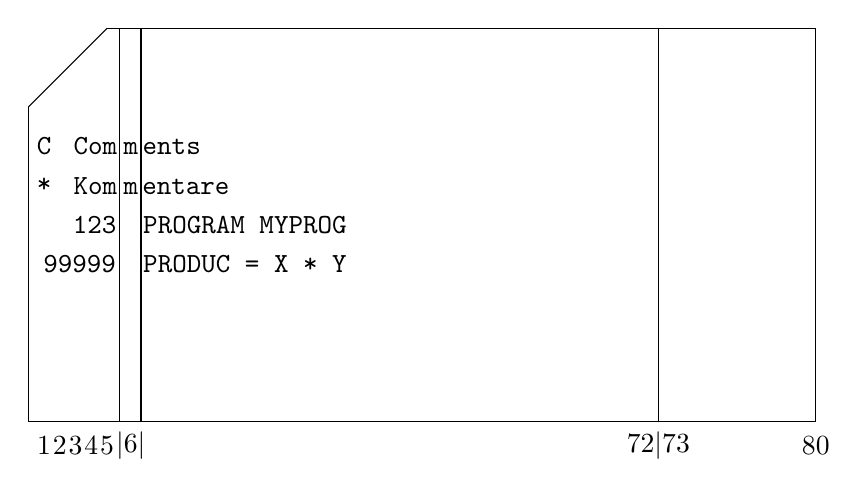
\begin{tikzpicture}
	\draw (0,0) -- (10,0);
	\draw (0,0) -- (0,4);
	\draw (0,4) -- (1,5);
	\draw (1,5) -- (10,5);
	\draw (10,0) -- (10,5);
	
	\node at (10,-0.3) (ende) {80};
	\node at (8,-0.3) (mitte) {$72\vert73$};
	\node at (0.2,-0.3) (1) {1};
	\node at (0.4,-0.3) (2) {2};
	\node at (0.6,-0.3) (3) {3};
	\node at (0.8,-0.3) (4) {4};
	\node at (1,-0.3) (5) {5};
	\node at (1.3,-0.3) (6) {$\vert 6\vert$};
	
	\draw (1.16,0) -- (1.16,5);
	\draw (1.43,0) -- (1.43,5);
	\draw (8,0) -- (8,5);
	
	\node at (0.2,3.5) (c) {\texttt{C}};
	\node at (0.85,3.5) (Com) {\texttt{Com}};
	\node at (1.3,3.47) (m) {\texttt{m}};
	\node at (1.82,3.488) (ents) {\texttt{ents}};
	
	\node at (0.2,3) (stern) {\texttt{*}};
	\node at (0.85,3) (Kom) {\texttt{Kom}};
	\node at (1.3,2.97) (m2) {\texttt{m}};
	\node at (2,2.99) (entare) {\texttt{entare}};
	
	\node at (0.84,2.5) (123) {\texttt{123}};
	\node at (2.75,2.5) (myprog) {\texttt{PROGRAM MYPROG}};
	\node at (0.65,2) (99999) {\texttt{99999}};
	\node at (2.75,2) (product) {\texttt{PRODUC = X * Y}};
\end{tikzpicture}
\end{document}